% Fig 2 — IRexp extraction & QC pipeline (hero schematic).
% Panel A: PMC OA + Chemotion -> IR extract -> Structure resolve -> Licence join
%          -> Release pools -> Final IRexp database, with cleaning-rules inset.
% Panel B: three illustrative automated QC rejection examples.
\documentclass[border=0pt,tikz]{standalone}
% Nature Portfolio / Scientific Data shared TikZ style for IRexp figures.
% Width: 183 mm double-column. Typography: Helvetica-class (phv).
\RequirePackage{tikz}
\RequirePackage{pgfplots}
\RequirePackage{xcolor}
\RequirePackage{helvet}
\IfFileExists{sansmathfonts.sty}{\RequirePackage{sansmathfonts}}{}
\renewcommand{\familydefault}{\sfdefault}
\pgfplotsset{compat=1.18}
\usetikzlibrary{
  arrows.meta,calc,positioning,fit,shapes.geometric,shapes.misc,
  backgrounds,shadows.blur,patterns,decorations.pathreplacing
}

% ---- Paul Tol / NMRexp-matched palette ----
\definecolor{nmrBlue}{HTML}{4A7EBB}
\definecolor{nmrBlueDark}{HTML}{2E5F8F}
\definecolor{nmrBlueLight}{HTML}{A8C8E8}
\definecolor{nmrPeach}{HTML}{E8B48C}
\definecolor{nmrNavy}{HTML}{1B3D5C}
\definecolor{nmrRed}{HTML}{C44E52}
\definecolor{nmrGreen}{HTML}{3D8B5E}
\definecolor{nmrOrange}{HTML}{D97B32}
\definecolor{ink}{HTML}{1A1A1A}
\definecolor{muted}{HTML}{7A7F85}
\definecolor{note}{HTML}{5C636A}
\definecolor{faint}{HTML}{E8EAEC}
\definecolor{ghost}{HTML}{C5C9CD}
\definecolor{tintBlue}{HTML}{EEF3F8}
\definecolor{tintGreen}{HTML}{EAF4EE}

\newcommand{\NatureFont}{\fontfamily{phv}\selectfont}
\newcommand{\PanelLabel}[1]{%
  {\NatureFont\bfseries\fontsize{8}{9.6}\selectfont #1}%
}
\newcommand{\FigBody}{\NatureFont\fontsize{7}{8.4}\selectfont}
\newcommand{\FigSmall}{\NatureFont\fontsize{5.5}{6.6}\selectfont}
\newcommand{\FigAxis}{\NatureFont\fontsize{7}{8.4}\selectfont}

\tikzset{
  nature arrow/.style={
    -{Latex[length=1.6mm,width=1.3mm]},
    line width=0.55pt, ink
  },
  nature arrow grey/.style={
    -{Latex[length=1.6mm,width=1.3mm]},
    line width=0.5pt, note
  },
  stage card/.style={
    draw=nmrBlueDark, line width=0.7pt, rounded corners=2.2pt,
    fill=white, inner sep=3pt, align=center, font=\FigBody
  },
  stage header/.style={
    fill=nmrBlueDark, text=white, font=\FigBody\bfseries,
    rounded corners=2.2pt, inner sep=2.5pt, align=center
  },
  soft card/.style={
    draw=ghost, line width=0.55pt, rounded corners=2.2pt,
    fill=white, inner sep=3.5pt, align=left, font=\FigBody
  },
}

\pgfplotsset{
  nature axis/.style={
    tick label style={font=\FigSmall, /pgf/number format/assume math mode},
    label style={font=\FigAxis\bfseries},
    title style={font=\FigBody\bfseries, color=ink},
    axis line style={ink, line width=0.5pt},
    tick style={ink, line width=0.45pt},
    major grid style={faint, line width=0.35pt},
    axis x line=bottom,
    axis y line=left,
    enlarge x limits=false,
    clip=false,
  },
  nature hbar/.style={
    nature axis,
    xbar,
    bar width=7pt,
    y=data,
    nodes near coords,
    every node near coord/.append style={
      font=\FigSmall, ink, anchor=west, /pgf/number format/fixed,
      /pgf/number format/1000 sep={,}
    },
    xtick=\empty,
    axis x line=none,
    y axis line style={ink, line width=0.55pt},
    ytick style={draw=none},
    y tick label style={font=\FigBody, ink, anchor=east},
    grid=major x,
    xmin=0,
  },
}


% ---------------------------------------------------------------------------
% Local drawing helpers (kept in this file only; shared style untouched)
% ---------------------------------------------------------------------------
\tikzset{
  pipe card/.style={
    draw=nmrBlueDark, line width=0.7pt, rounded corners=1.6pt, fill=white
  },
  pipe header/.style={
    fill=nmrBlueDark, rounded corners=1.6pt
  },
  step badge/.style={
    circle, draw=nmrNavy, fill=nmrNavy, line width=0.6pt,
    minimum size=5.6mm, inner sep=0
  },
}

\begin{document}
\NatureFont
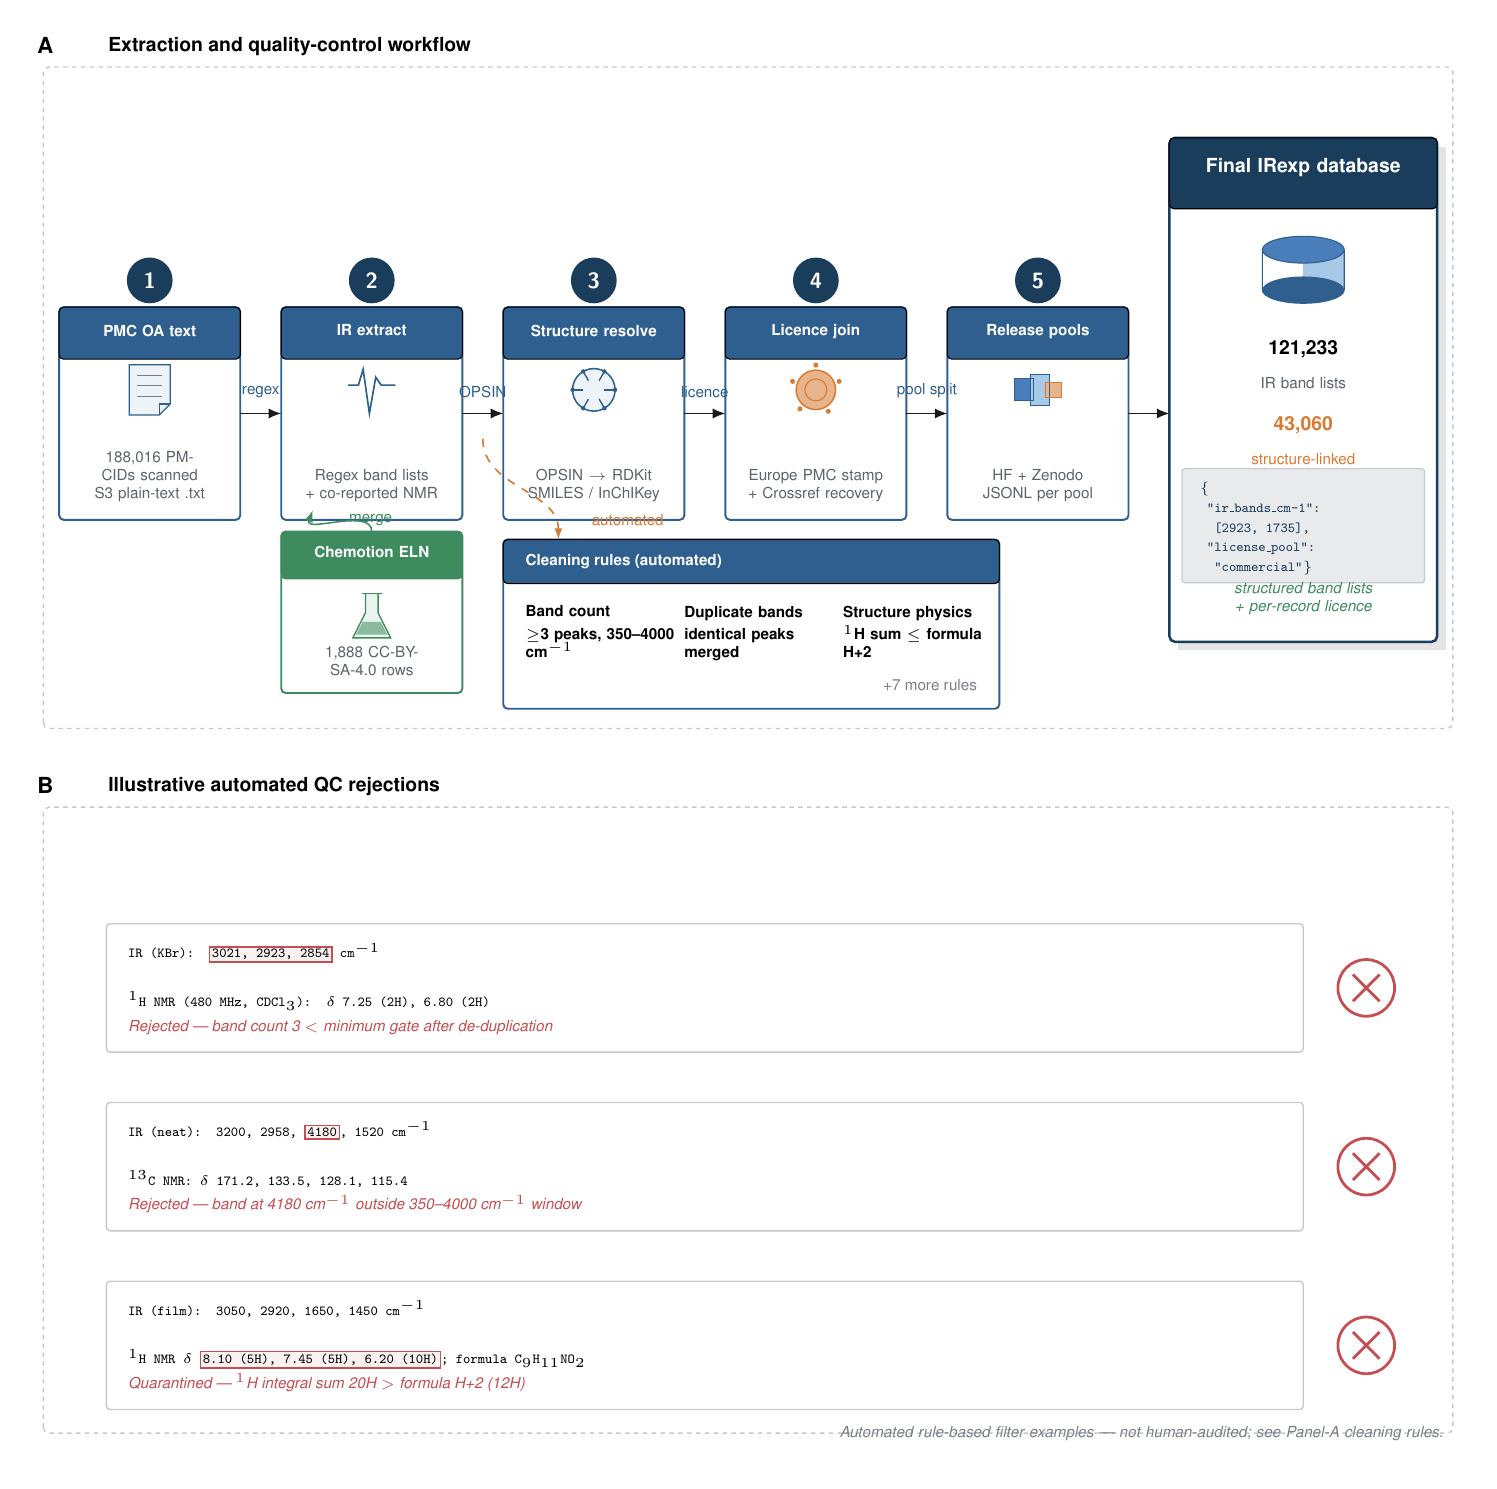
\begin{tikzpicture}[x=1mm,y=1mm]

\useasboundingbox (0,0) rectangle (183,182);

% ===========================================================================
% Shared numeric geometry — Panel A
% ===========================================================================
\def\CW{23}      % normal stage card width
\def\CH{27}      % normal stage card height
\def\CTop{146.5} % main-row card top y
\def\CBot{119.5} % main-row card bottom y (= \CTop-\CH)
\def\Gap{5.2}     % horizontal gap between stage cards
\def\MidY{133}   % vertical centre of main row (for connector arrows)

\pgfmathsetmacro{\SxA}{4}
\pgfmathsetmacro{\SxB}{\SxA+\CW+\Gap}
\pgfmathsetmacro{\SxC}{\SxB+\CW+\Gap}
\pgfmathsetmacro{\SxD}{\SxC+\CW+\Gap}
\pgfmathsetmacro{\SxE}{\SxD+\CW+\Gap}
\pgfmathsetmacro{\SxF}{\SxE+\CW+\Gap}   % hero card left
\def\HW{34}      % hero card width
\def\HTop{168}
\def\HBot{104}

% ===========================================================================
% Panel label
% ===========================================================================
\node[anchor=north west] at (0,182) {\PanelLabel{A}};
\node[font=\FigAxis,anchor=north west] at (9,182) {\bfseries Extraction and quality-control workflow};

% ===========================================================================
% Panel A outer boundary (very light, organisational only)
% ===========================================================================
\draw[ghost, line width=0.5pt, dash pattern=on 1.6pt off 1.6pt, rounded corners=2pt]
  (2,93) rectangle (181,177);

% ===========================================================================
% Stage-card macro: \Stage{x}{caption-top}{caption-bottom}{step number}
% ===========================================================================
\newcommand{\Stage}[4]{%
  \begin{scope}[shift={(#1,\CBot)}]
    \draw[pipe card] (0,0) rectangle (\CW,\CH);
    \draw[pipe header] (0,\CH-6.6) rectangle (\CW,\CH);
    \node[font=\FigSmall,text=white,align=center,anchor=north,text width=22mm]
      at (\CW/2,\CH-1.0) {\bfseries #2};
    \node[font=\FigSmall,text=note,align=center,anchor=south,text width=21mm]
      at (\CW/2,1.0) {#3};
  \end{scope}
  \node[step badge] at (#1+\CW/2,\CTop+3.4) {\color{white}\footnotesize\bfseries #4};
}

% ---------------------------------------------------------------------------
% Icons (drawn at local origin (0,0), ~8mm bounding box), placed per stage
% ---------------------------------------------------------------------------
\newcommand{\IconPDF}{%
  \draw[nmrBlueDark,line width=0.45pt,fill=tintBlue]
    (-2.6,-3.2) -- (1.2,-3.2) -- (2.6,-1.8) -- (2.6,3.2) -- (-2.6,3.2) -- cycle;
  \draw[nmrBlueDark,line width=0.4pt] (1.2,-3.2) -- (1.2,-1.8) -- (2.6,-1.8);
  \foreach \yy in {-0.8,0.5,1.8} {\draw[muted,line width=0.35pt] (-1.6,\yy) -- (1.6,\yy);}
}
\newcommand{\IconSpectrum}{%
  \draw[nmrBlueDark,line width=0.6pt]
    (-3.0,0.6) -- (-1.7,0.6) -- (-1.1,2.6) -- (-0.3,-3.0) -- (0.5,1.6) -- (1.2,0.6) -- (3.0,0.6);
}
\newcommand{\IconHexagon}{%
  \draw[nmrBlueDark,line width=0.55pt,fill=tintBlue] (0,0) circle [radius=2.7mm];
  \foreach \ang in {0,60,...,300}{
    \draw[nmrBlueDark,line width=0.5pt] (\ang:1.35mm) -- (\ang:2.7mm);
    \fill[nmrBlueDark] (\ang:2.7mm) circle (0.28mm);
  }
}
\newcommand{\IconSeal}{%
  \draw[nmrOrange,line width=0.55pt,fill=nmrPeach] (0,0) circle [radius=2.5mm];
  \draw[nmrOrange,line width=0.4pt] (0,0) circle [radius=1.4mm];
  \foreach \ang in {20,90,160,230,300}{\fill[nmrOrange] (\ang:3.15mm) circle (0.32mm);}
}
\newcommand{\IconPools}{%
  \fill[nmrBlue] (-3.0,-1.4) rectangle (-0.6,1.4);
  \fill[nmrBlueLight] (-1.0,-2.0) rectangle (1.4,2.0);
  \fill[nmrPeach] (1.0,-1.0) rectangle (3.0,1.0);
  \draw[nmrBlueDark,line width=0.3pt] (-3.0,-1.4) rectangle (-0.6,1.4);
  \draw[nmrBlueDark,line width=0.3pt] (-1.0,-2.0) rectangle (1.4,2.0);
  \draw[nmrOrange,line width=0.3pt] (1.0,-1.0) rectangle (3.0,1.0);
}
\newcommand{\IconFlask}{%
  \draw[nmrGreen,line width=0.5pt,fill=tintGreen]
    (-0.8,3.0) -- (-0.8,0.6) -- (-2.4,-2.6) -- (2.4,-2.6) -- (0.8,0.6) -- (0.8,3.0);
  \draw[nmrGreen,line width=0.5pt] (-1.3,3.0) -- (1.3,3.0);
  \fill[nmrGreen,opacity=0.55] (-2.0,-2.2) -- (2.0,-2.2) -- (1.15,-0.55) -- (-1.15,-0.55) -- cycle;
}

% ===========================================================================
% Main-row stage cards
% ===========================================================================
\Stage{\SxA}{PMC OA text}{188,016 PMCIDs scanned\\S3 plain-text .txt}{1}
\begin{scope}[shift={(\SxA+\CW/2,\CBot+16.5)}]\IconPDF\end{scope}

\Stage{\SxB}{IR extract}{Regex band lists\\+ co-reported NMR}{2}
\begin{scope}[shift={(\SxB+\CW/2,\CBot+16.5)}]\IconSpectrum\end{scope}

\Stage{\SxC}{Structure resolve}{OPSIN $\to$ RDKit\\SMILES / InChIKey}{3}
\begin{scope}[shift={(\SxC+\CW/2,\CBot+16.5)}]\IconHexagon\end{scope}

\Stage{\SxD}{Licence join}{Europe PMC stamp\\+ Crossref recovery}{4}
\begin{scope}[shift={(\SxD+\CW/2,\CBot+16.5)}]\IconSeal\end{scope}

\Stage{\SxE}{Release pools}{HF + Zenodo\\JSONL per pool}{5}
\begin{scope}[shift={(\SxE+\CW/2,\CBot+16.5)}]\IconPools\end{scope}

% ---------------------------------------------------------------------------
% Chemotion ELN branch (merges into IR extract)
% ---------------------------------------------------------------------------
\def\ChX{\SxB}
\def\ChY{97.5}
\def\ChW{23}
\def\ChH{20.5}
\draw[nmrGreen, line width=0.7pt, rounded corners=1.6pt, fill=white]
  (\ChX,\ChY) rectangle (\ChX+\ChW,\ChY+\ChH);
\draw[nmrGreen, rounded corners=1.6pt, fill=nmrGreen]
  (\ChX,\ChY+\ChH-6.0) rectangle (\ChX+\ChW,\ChY+\ChH);
\node[font=\FigSmall,text=white,align=center,anchor=north,text width=22mm]
  at (\ChX+\ChW/2,\ChY+\ChH-0.6) {\bfseries Chemotion ELN};
\begin{scope}[shift={(\ChX+\ChW/2,\ChY+9.6)}]\IconFlask\end{scope}
\node[font=\FigSmall,text=note,align=center,anchor=south,text width=21mm]
  at (\ChX+\ChW/2,\ChY+0.9) {1,888 CC-BY-SA-4.0 rows};
\draw[nature arrow, nmrGreen, -{Latex[length=1.5mm,width=1.1mm]}]
  (\ChX+\ChW/2,\ChY+\ChH) to[out=90,in=250] node[midway,right,font=\FigSmall,text=nmrGreen]{merge} (\SxB+4,\CBot+1.2);

% ---------------------------------------------------------------------------
% Inter-stage arrows (main row) with small regex/rule captions
% ---------------------------------------------------------------------------
\newcommand{\Flow}[3]{%
  \draw[nature arrow] (#1,\MidY) -- (#2,\MidY);
  \node[font=\FigSmall,text=nmrBlueDark,anchor=south] at ({(#1+#2)/2},\MidY+0.8) {#3};
}
\Flow{\SxA+\CW}{\SxB}{regex}
\Flow{\SxB+\CW}{\SxC}{OPSIN}
\Flow{\SxC+\CW}{\SxD}{licence}
\Flow{\SxD+\CW}{\SxE}{pool split}
\draw[nature arrow] (\SxE+\CW,\MidY) -- (\SxF,\MidY);

% ---------------------------------------------------------------------------
% Cleaning-rules inset (branches from the extract -> resolve arrow)
% ---------------------------------------------------------------------------
\pgfmathsetmacro{\CleanBranchX}{\SxB+\CW+\Gap/2}
\def\CRx{\SxC}
\def\CRy{95.5}
\def\CRw{63}
\def\CRh{21.5}
\draw[nmrOrange, line width=0.6pt, dashed, -{Latex[length=1.4mm,width=1.0mm]}]
  (\CleanBranchX,\MidY-3.2) to[out=270,in=90] (\CRx+7,\CRy+\CRh);
\node[font=\FigSmall,text=nmrOrange,anchor=south west] at (\CRx+10,\CRy+\CRh+0.5) {automated};

\draw[nmrBlueDark, line width=0.7pt, rounded corners=1.6pt, fill=white]
  (\CRx,\CRy) rectangle (\CRx+\CRw,\CRy+\CRh);
\draw[pipe header] (\CRx,\CRy+\CRh-5.6) rectangle (\CRx+\CRw,\CRy+\CRh);
\node[font=\FigSmall,text=white,anchor=west] at (\CRx+1.6,\CRy+\CRh-2.8) {\bfseries Cleaning rules (automated)};
\pgfmathsetmacro{\CRcolw}{(\CRw-4)/3}
\foreach \i/\lab/\rule in {
  0/{Band count}/{$\geq$3 peaks, 350--4000 cm$^{-1}$},
  1/{Duplicate bands}/{identical peaks merged},
  2/{Structure physics}/{$^1$H sum $\le$ formula H+2}
}{
  \pgfmathsetmacro{\cx}{\CRx+1.6+\i*(\CRcolw+0.5)}
  \node[font=\FigSmall,anchor=north west,align=left,text width=\CRcolw mm]
    at (\cx,\CRy+\CRh-7.2) {\bfseries\lab\\[1.5pt]\rule};
}
\node[font=\FigSmall,text=muted,anchor=south east,align=right] at (\CRx+\CRw-1.6,\CRy+1.0) {+7 more rules};

% ===========================================================================
% Final IRexp hero card
% ===========================================================================
% soft shadow (offset rect)
\fill[ghost,opacity=0.5] ($(\SxF,\HBot)+(1.1,-1.1)$) rectangle ($(\SxF+\HW,\HTop)+(1.1,-1.1)$);
\draw[nmrNavy, line width=0.9pt, rounded corners=2pt, fill=white]
  (\SxF,\HBot) rectangle (\SxF+\HW,\HTop);
\draw[pipe header,fill=nmrNavy] (\SxF,\HTop-9.0) rectangle (\SxF+\HW,\HTop);
\node[font=\FigBody,text=white,anchor=north,align=center,text width=32mm]
  at (\SxF+\HW/2,\HTop-1.4) {\bfseries Final IRexp database};

% DB cylinder icon
\begin{scope}[shift={(\SxF+\HW/2,152.5)}]
  \fill[nmrBlueLight] (0,-3.8) rectangle (5.2,1.3);
  \fill[nmrBlue] (0,1.3) ellipse (5.2mm and 1.7mm);
  \fill[nmrBlueDark] (0,-3.8) ellipse (5.2mm and 1.7mm);
  \draw[nmrBlueDark,line width=0.4pt] (-5.2,1.3) -- (-5.2,-3.8) arc (180:360:5.2mm and 1.7mm) -- (5.2,1.3);
  \draw[nmrBlueDark,line width=0.4pt] (0,1.3) ellipse (5.2mm and 1.7mm);
\end{scope}

\node[font=\FigBody,anchor=north,align=center,text width=32mm] at (\SxF+\HW/2,143.5)
  {\bfseries 121,233}; 
\node[font=\FigSmall,text=note,anchor=north,align=center,text width=32mm] at (\SxF+\HW/2,138.8)
  {IR band lists};
\node[font=\FigBody,anchor=north,text=nmrOrange,align=center,text width=32mm] at (\SxF+\HW/2,133.8)
  {\bfseries 43,060};
\node[font=\FigSmall,text=nmrOrange,anchor=north,align=center,text width=32mm] at (\SxF+\HW/2,129.1)
  {structure-linked};

% JSON snippet (manual line breaks; no forced text width to avoid tt-font
% ligature/brace width mis-measurement and overfull boxes)
\draw[ghost,line width=0.4pt,fill=faint,rounded corners=1pt]
  (\SxF+1.6,111.5) rectangle (\SxF+\HW-1.6,126.0);
\node[font=\FigSmall,anchor=north west,align=left,text=nmrNavy] at (\SxF+2.6,125.5)
  {\texttt{\{}\\[0.5pt]\texttt{\ "ir\_bands\_cm-1":}\\[0.5pt]\texttt{\ \ [2923, 1735],}\\[0.5pt]\texttt{\ "license\_pool":}\\[0.5pt]\texttt{\ \ "commercial"\}}};

\node[font=\FigSmall,text=nmrGreen,anchor=south,align=center,text width=32mm] at (\SxF+\HW/2,\HBot+2.2)
  {\itshape structured band lists + per-record licence};

% ===========================================================================
% Panel B — QC rejection examples
% ===========================================================================
\def\PBTop{88}
\node[anchor=north west] at (0,\PBTop) {\PanelLabel{B}};
\node[font=\FigAxis,anchor=north west] at (9,\PBTop) {\bfseries Illustrative automated QC rejections};

\draw[ghost, line width=0.5pt, dash pattern=on 1.6pt off 1.6pt, rounded corners=2pt]
  (2,3.5) rectangle (181,\PBTop-5);

\newcommand{\XMark}[2]{%
  \begin{scope}[shift={(#1,#2)}]
    \draw[nmrRed,line width=1.0pt] (0,0) circle [radius=3.6mm];
    \draw[nmrRed,line width=1.0pt] (-1.7,-1.7) -- (1.7,1.7);
    \draw[nmrRed,line width=1.0pt] (-1.7,1.7) -- (1.7,-1.7);
  \end{scope}
}

% Row geometry
\def\RowH{20.5}
\def\RowGap{2.2}
\pgfmathsetmacro{\RowThreeY}{6.5}
\pgfmathsetmacro{\RowTwoY}{\RowThreeY+\RowH+\RowGap}
\pgfmathsetmacro{\RowOneY}{\RowTwoY+\RowH+\RowGap}

% Inline highlight for the offending token: a real \fcolorbox drawn by TeX
% around the exact text, so it is always pixel-perfectly aligned (no manual
% coordinate guessing over monospace glyph widths).
\setlength{\fboxsep}{0.6pt}\setlength{\fboxrule}{0.5pt}
\newcommand{\Flag}[1]{\fcolorbox{nmrRed}{nmrRed!8}{\ttfamily #1}}

\newcommand{\QCRow}[4]{%
  % #1 = y (bottom), #2 = ir/nmr line 1 (may contain \Flag), #3 = line 2, #4 = reason text
  \draw[ghost, line width=0.5pt, rounded corners=1.3pt, fill=white]
    (10,#1) rectangle (162,#1+\RowH-4.2);
  \node[font=\FigSmall,anchor=north west,align=left] at (11.5,#1+\RowH-5.4) {\ttfamily #2};
  \node[font=\FigSmall,anchor=north west,align=left] at (11.5,#1+\RowH-11.6) {\ttfamily #3};
  \node[font=\FigSmall,text=nmrRed,anchor=south west,align=left] at (11.5,#1+1.0) {\itshape #4};
  \pgfmathsetmacro{\qcMarkY}{#1+(\RowH-4.2)/2}
  \XMark{170}{\qcMarkY}
}

% Row 1 — band count too low after gate (whole 3-band list flagged)
\QCRow{\RowOneY}{IR (KBr): \Flag{3021, 2923, 2854} cm$^{-1}$}{$^1$H NMR (480 MHz, CDCl$_3$): $\delta$ 7.25 (2H), 6.80 (2H)}{Rejected --- band count 3 $<$ minimum gate after de-duplication}

% Row 2 — single band outside physical IR window
\QCRow{\RowTwoY}{IR (neat): 3200, 2958, \Flag{4180}, 1520 cm$^{-1}$}{$^{13}$C NMR: $\delta$ 171.2, 133.5, 128.1, 115.4}{Rejected --- band at 4180 cm$^{-1}$ outside 350--4000 cm$^{-1}$ window}

% Row 3 — integral / formula mismatch (flag the integral list, not the formula)
\QCRow{\RowThreeY}{IR (film): 3050, 2920, 1650, 1450 cm$^{-1}$}{$^1$H NMR $\delta$ \Flag{8.10 (5H), 7.45 (5H), 6.20 (10H)}; formula C$_9$H$_{11}$NO$_2$}{Quarantined --- $^1$H integral sum 20H $>$ formula H+2 (12H)}

\node[font=\FigSmall,text=muted,anchor=south east,align=right,text width=90mm] at (181,1.3)
  {\itshape Automated rule-based filter examples --- not human-audited; see Panel-A cleaning rules.};

\end{tikzpicture}
\end{document}
